\Variant{07.03.2026 (2-smena)}
\QQ{1}{Agar $m=24^3\cdot6^{12}\cdot20^3$ bölsa, $\dfrac{m^2}{2^n}$ kasrning qiymati natural son böladigan $n$ ning eng katta qiymatini toping.
\Opts{$54$}{$48$}{$27$}{$60$}}
\QQ{2}{Agar $x\in\left[\dfrac12;\,2\right]$ bölsa, $\bigl||3x-1|-|x|\bigr|-|x-2|$ ifodani soddalaştiring.
\Opts{$x$}{$3(x-1)$}{$0$}{$3$}}
\QQ{3}{Ikkita kenguru orasidagi masofa $30$ metr (katta kenguru kiçigini quvmoqda). Katta kenguru bir sakraşda $2$ metr, kiçigi $1$ metr sakraydi va katta kenguru ikki marta sakraganda kiçigi uç marta sakraydi. Katta kenguru kiçigini quvib yetgunça qança masofa bosib ötadi?
\Opts{$120$}{$180$}{$90$}{$60$}}
\QQ{4}{Uç nafar işçi birgalikda $4\,080\,000$ söm iş haqi oldi. Birinçi işçi olgan pulning ikkinçi işçi olgan pulga nisbati $7\frac12:\frac74$ ga teng, uçinçi işçi esa birinçi işçi olgan pulning $43\frac13\%$ qismini oldi. Uçinçi işçi neça söm olgan?
\Opts{$1\,060\,800$}{$1\,080\,600$}{$2\,440\,000$}{$571\,000$}}
\QQ{5}{Eng katta sonni toping.
\Opts{$2^{2^{2^2}}$}{$2^{2^{22}}$}{$2^{222}$}{$2^{22^2}$}}
\QQ{6}{Hisoblang:
\[\sqrt2\left(\sqrt5-1\right)\left(3+\sqrt5\right)\sqrt{3-\sqrt5}\]
\Opts{$16$}{$2$}{$4$}{$8$}}
\QQ{7}{Soddalaştiring:
\[\sqrt[3]{\frac{125\cdot x^{\frac65}}{54}}\]
\Opts{$\dfrac{5\sqrt[3]4\,x^{\frac25}}6$}{$\dfrac{5\sqrt[3]4\,x^{\frac35}}6$}{$\dfrac{5\sqrt[3]2\,x^{\frac25}}6$}{$\dfrac{5\sqrt[3]2\,x^{\frac35}}6$}}
\QQ{8}{Arifmetik progressiyada $a_5=5$ va $a_7\cdot a_{10}$ eng kiçik qiymatga ega bölsa, $d$ ni toping.
\Opts{$-0{,}75$}{$-2{,}25$}{$-1{,}25$}{$-1{,}75$}}
\QQ{9}{$\{a_n\}$ arifmetik progressiya va $\{b_n\}$ geometrik progressiya berilgan. Agar $b_1+b_2+b_3=16$, $b_1=a_2$, $b_2=a_4$, $b_3=a_6$ va $a_1+a_2+a_3+\ldots+a_n=176$ bölsa, $n$ ni toping.
\Opts{$11$}{$32$}{$33$}{$36$}}
\QQ{10}{Soddalaştiring:
\[\frac{a^3-b^3}{(2a+b)^2-3a(a+b)}+\frac{\left(a^2+b\right)\left(b^2+a\right)-ab(ab+1)}{a^2-ab+b^2}\]
\Opts{$2b$}{$2a-2b$}{$2a+2b$}{$2a$}}
\QQ{11}{Agar $a^3+a-1=0$ bölsa, $\dfrac{a^4+a^3+a^2+9}{a^5-a^2-a+6}$ ni toping.
\Opts{$2$}{$\dfrac23$}{$1$}{$\dfrac53$}}
\QQ{12}{Hisoblang:
\[\frac{3\sin10^\circ-\sqrt3\cos10^\circ}{3\cos70^\circ}\]
\Opts{$\dfrac2{\sqrt3}$}{$-\dfrac2{\sqrt3}$}{$\dfrac{\sqrt2}3$}{$-\dfrac{\sqrt2}3$}}
\QQ{13}{$\alpha$, $\beta$ va $\gamma$ — uçburçakning içki burçaklari. Agar $\sin\alpha\sin\beta\sin\gamma=\dfrac12$ bölsa, $\sin2\alpha+\sin2\beta+\sin2\gamma$ ni toping.
\Opts{$2$}{$\dfrac{\sqrt3}2$}{$0$}{$1$}}
\QQ{14}{Tenglama neçta haqiqiy ildizga ega?
\[\frac{7^x-11^x}{\sqrt{77^x-121^x}}=1\]
\Opts{$2$}{$1$}{ildizga ega emas}{çeksiz köp}}
\QQ{15}{Tengsizlikni neçta butun son qanoatlantiradi?
\[\log_{\frac12}\left(2x-5\frac12\right)\ge\log_{4-x}1\]
\Opts{$1$}{$2$}{çeksiz köp}{butun yeçimga ega emas}}
\QQ{16}{$x^2-3x+a^2=0$ tenglama haqiqiy ildizga ega böladigan $a$ ning neçta butun qiymati mavjud?
\Opts{$1$}{$2$}{$3$}{$4$}}
\QQ{17}{Tenglamaning haqiqiy ildizlari yiğindisini (agar u bitta bölsa, şu ildizni) toping:
\[\sqrt[3]{(x+3)^2}-6\sqrt[3]{(x-3)^2}=\sqrt[3]{9-x^2}\]
\Opts{$2\dfrac{11}{14}$}{$9$}{$6\dfrac9{14}$}{$0$}}
\QQ{18}{Tengsizlikni qanoatlantiradigan butun yeçimlar yiğindisini toping:
\[\frac{x^2+3x+46}{x^2-7x+10}\le\frac8{5-x}\]
\Opts{$-12$}{$7$}{$5$}{$-4$}}
\QQ{19}{Tengsizlikni yeçing:
\[\sqrt{x-11}+\sqrt{12-x}>0\]
\Opts{$(11;\,12)$}{$[11;\,12]$}{$\{11;\,12\}$}{$(-\infty;\,\infty)$}}
\QQ{20}{Funksiyaning aniqlaniş sohasiga tegişli bölgan butun sonlar yiğindisini toping:
\[f(x)=\frac{\sqrt{x+3}-\sqrt{6-x}}{x^2-10x+25}\]
\Opts{$10$}{$13$}{$7$}{$15$}}
\QQ{21}{Aniqmas integralni hisoblang:
\[\int\frac{dx}{x^3+1}\]
\Opts{$\dfrac13\ln|x+1|-\dfrac12\ln\left(x^2-x+1\right)+\sqrt3\arctg\dfrac{x-\frac12}{2\sqrt3}+C$}{$\dfrac13\ln|x+1|-\ln\left(x^2-x+1\right)-\sqrt3\arctg\dfrac{x-1}{\sqrt3}+C$}{$\dfrac13\ln|x+1|-\dfrac16\ln\left(x^2-x+1\right)+\dfrac1{\sqrt3}\arctg\dfrac{2x-1}{\sqrt3}+C$}{$\dfrac13\ln|x+1|+\dfrac12\ln\left(x^2-x+1\right)+\sqrt3\arctg\dfrac{2x-1}{\sqrt3}+C$}}
\QQ{22}{Agar $f(x)=\dfrac{x+x^2+x^3+\ldots+x^{2024}}{x+x^2+x^3+\ldots+x^{1012}}$ bölsa, $f'(1)$ ni toping.
\Opts{$1$}{$-1$}{$-1012$}{$1012$}}
\QQ{23}{Radiusi $1+\sqrt2$ ga teng bölgan çorak doiraga $O_1$ markazli aylana içki çizilgan. $O_1$ markazli aylana radiusini toping.
\qfig{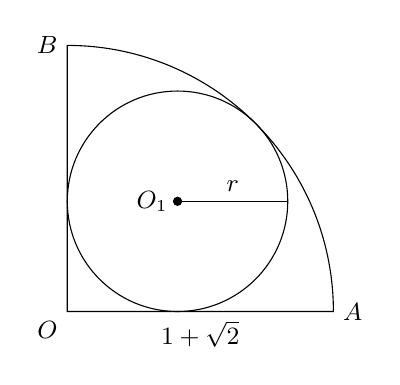
\begin{tikzpicture}[scale=1.4,font=\small]
\draw (0,0)--(2.414,0) arc (0:90:2.414)--cycle; \draw (1,1) circle (1); \draw (1,1)--(2,1); \fill (1,1) circle (1.2pt);
\node[below left] at (0,0) {$O$}; \node[right] at (2.414,0) {$A$}; \node[left] at (0,2.414) {$B$}; \node[left] at (1,1) {$O_1$}; \node[above] at (1.5,1) {$r$};
\node[below] at (1.207,0) {$1+\sqrt2$};
\end{tikzpicture}}
\Opts{$\sqrt2$}{$1$}{$\sqrt3$}{$\dfrac{\sqrt2}2$}}
\QQ{24}{$f(x)=x^2-ax+3$ va $g(x)=2x-1$ funksiyalar grafiklari bitta nuqtada kesişadigan $a$ ning barça qiymatlari yiğindisini toping (agar u bitta bölsa, şu $a$ ni toping).
\Opts{$2$}{$-4$}{$4$}{$6$}}
\QQ{25}{Uçburçakning ikkita içki burçagi $64^\circ$ va $76^\circ$ ga teng. Uçburçak bissektrisalarining kesişişidan hosil bölgan eng kiçik burçakni toping.
\qfig{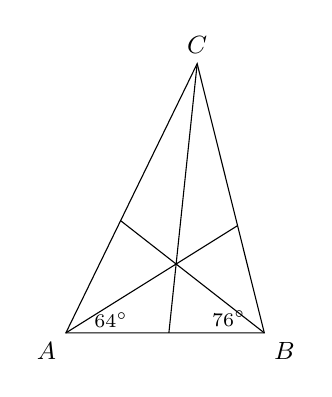
\begin{tikzpicture}[scale=0.36,font=\small]
\coordinate (A) at (0,0); \coordinate (B) at (7,0); \coordinate (C) at (4.632,9.497);
\draw (A)--(B)--(C)--cycle; \draw (A)--(6.056,3.784); \draw (B)--(1.931,3.960); \draw (C)--(3.634,0);
\node[below left] at (A) {$A$}; \node[below right] at (B) {$B$}; \node[above] at (C) {$C$};
\node at (1.6,0.45) {\scriptsize$64^\circ$}; \node at (5.75,0.5) {\scriptsize$76^\circ$};
\end{tikzpicture}}
\Opts{$52^\circ$}{$58^\circ$}{$70^\circ$}{$40^\circ$}}
\QQ{26}{$ABC$ uçburçakda $AB=8$, $BC=13$ va $AC=15$. Agar $L$ nuqta uçburçak bissektrisalarining kesişiş nuqtasi, $M$ nuqta medianalarining kesişiş nuqtasi bölsa, $LM$ kesma uzunligini toping.
\qfig{\begin{tikzpicture}[scale=0.45,font=\small]
\coordinate (A) at (0,0); \coordinate (C) at (15,0); \coordinate (B) at (4,6.928); \coordinate (L) at (5,2.887); \coordinate (M) at (6.333,2.309);
\draw (A)--(B)--(C)--cycle; \draw (L)--(M); \fill (L) circle (3pt); \fill (M) circle (3pt);
\node[below left] at (A) {$A$}; \node[above] at (B) {$B$}; \node[below right] at (C) {$C$}; \node[above left] at (L) {$L$}; \node[below right] at (M) {$M$};
\node[above left] at (2,3.464) {$8$}; \node[above right] at (9.5,3.464) {$13$}; \node[below] at (7.5,0) {$15$};
\end{tikzpicture}}
\Opts{$\dfrac{2\sqrt5}3$}{$\dfrac{\sqrt{19}}3$}{$\dfrac{\sqrt{17}}3$}{$\dfrac{\sqrt7}3$}}
\QQ{27}{Rasmdagi maʼlumotlar asosida $ABCD$ kvadratning yuzini toping.
\qfig{\begin{tikzpicture}[scale=0.42,font=\small]
\coordinate (A) at (0,0); \coordinate (B) at (0,8.944); \coordinate (C) at (8.944,8.944); \coordinate (D) at (8.944,0);
\coordinate (P1) at (2.236,4.472); \coordinate (P2) at (4.025,5.367); \coordinate (P3) at (5.814,1.789); \coordinate (P4) at (7.603,2.683);
\draw (A)--(B)--(C)--(D)--cycle; \draw (B)--(P1)--(P2)--(P3)--(P4)--(D);
\foreach \p/\a/\b in {P1/B/P2,P2/P1/P3,P3/P2/P4,P4/P3/D} \draw ($(\p)!0.42cm!(\a)$)--($(\p)!0.42cm!(\a)+(\p)!0.42cm!(\b)-(\p)$)--($(\p)!0.42cm!(\b)$);
\node[below left] at (A) {$A$}; \node[above left] at (B) {$B$}; \node[above right] at (C) {$C$}; \node[below right] at (D) {$D$};
\node[left] at (1.1,6.6) {$5$}; \node[above] at (3.0,5.0) {$2$}; \node[right] at (5.0,3.7) {$4$}; \node[above] at (6.6,2.35) {$2$}; \node[right] at (8.3,1.4) {$3$};
\end{tikzpicture}}
\Opts{$100$}{$80$}{$81$}{$40$}}
\QQ{28}{Aylanaga muntazam oltiburçak içki va taşqi çizilgan. Taşqi çizilgan muntazam oltiburçak yuzining içki çizilgan muntazam oltiburçak yuziga nisbatini toping.
\qfig{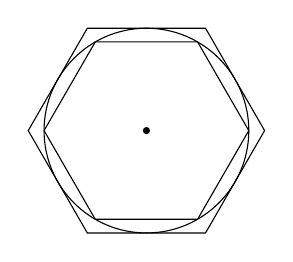
\begin{tikzpicture}[scale=1.3,font=\small]
\draw (0,0) circle (1);
\draw (1,0)--(0.5,0.866)--(-0.5,0.866)--(-1,0)--(-0.5,-0.866)--(0.5,-0.866)--cycle;
\draw (1.1547,0)--(0.5774,1)--(-0.5774,1)--(-1.1547,0)--(-0.5774,-1)--(0.5774,-1)--cycle;
\fill (0,0) circle (1pt);
\end{tikzpicture}}
\Opts{$\dfrac32$}{$\dfrac43$}{$\dfrac54$}{$\dfrac65$}}
\QQ{29}{$\overrightarrow{AB}$ vektorning boşi $A(6;\,4;\,-2)$ nuqtada, oxiri $B$ esa $Oxy$ tekisligida yotadi. $\overrightarrow{CD}(4;\,-3;\,1)$ vektor $\overrightarrow{AB}$ vektorga kollinear bölsa, $\overrightarrow{AB}$ vektor koordinatalari yiğindisini toping.
\Opts{$4$}{$-12$}{$-4$}{$12$}}
\QQ{30}{Silindr öq kesimining diagonali asos radiusidan $4$ marta katta. Silindr yon sirtining yuzi $12\sqrt3\pi$ bölsa, silindr hajmini toping.
\Opts{$12\pi$}{$24\pi$}{$18\pi$}{$54\pi$}}
\QQ{31}{Rasmda böyalgan töplamni aniqlang.
\qfig{\begin{tikzpicture}[scale=0.75,font=\small]
\begin{scope}\clip (-0.66,0) circle (1); \clip (0,-1.02) circle (1); \fill[qfill,even odd rule] (-3,-3) rectangle (3,3) (0.66,0) circle (1); \end{scope}
\draw (-0.66,0) circle (1); \draw (0.66,0) circle (1); \draw (0,-1.02) circle (1);
\node at (-1.05,0.4) {$A$}; \node at (1.05,0.4) {$B$}; \node at (0,-1.5) {$C$};
\end{tikzpicture}}
\Opts{$(A\cap C)\setminus B$}{$B\setminus(A\cap C)$}{$B\setminus(A\cup C)$}{$(A\cup C)\setminus B$}}
\QQ{32}{Raqamlari yiğindisi $9$ ga teng bölgan neçta uç xonali son bor?
\Opts{$36$}{$45$}{$44$}{$48$}}
\QQ{33}{\Moslash{Konus asosiga tomoni $4$ cm bölgan $ABED$ kvadrat içki çizilgan. Konusning $S$ uçi kvadratning $A$ va $B$ uçlari bilan tutaştirilib, $ABS$ uçburçak kesim hosil qilindi. Bu kesimda $SA$ va $SB$ yasovçilar orasidagi burçak $60^\circ$ ga teng.
\par\centering\begin{tikzpicture}[scale=0.62,font=\small]
\coordinate (S) at (0,4.2); \coordinate (A) at (-2.819,-0.274); \coordinate (B) at (1.026,-0.752); \coordinate (E) at (2.819,0.274); \coordinate (D) at (-1.026,0.752);
\fill[qfill] (S)--(A)--(B)--cycle;
\draw (3,0) arc (0:-180:3 and 0.8); \draw[dashed] (3,0) arc (0:180:3 and 0.8);
\draw (S)--(-3,0); \draw (S)--(3,0); \draw (S)--(A); \draw (S)--(B); \draw[dashed] (S)--(0,0);
\draw (A)--(B)--(E); \draw[dashed] (E)--(D)--(A); \fill (0,0) circle (1.5pt);
\draw ($(S)!0.8cm!(A)$) arc[start angle=237.9,end angle=282.4,radius=0.8cm]; \node at ($(S)+(260:1.2)$) {\scriptsize$60^\circ$};
\node[above] at (S) {$S$}; \node[left] at (A) {$A$}; \node[below] at (B) {$B$}; \node[right] at (E) {$E$}; \node[above left] at (D) {$D$}; \node[below right] at ($(B)!0.5!(E)$) {$4$};
\end{tikzpicture}}{A) $16\sqrt2$\par B) $8\sqrt2$\par C) $2\sqrt2$\par D) $4\sqrt2$\par E) $4\sqrt3$\par F) $2\sqrt3$}{Konus balandligini toping (cm).}{$ABS$ kesim yuzini toping (cm$^2$).}{Konus hajmini toping (cm$^3$) ($\pi\approx3$ deb olinsin).}}
\QQ{36}{Tenglamalar sistemasi berilgan:
\[\begin{cases}x^4+y^4=17(x-y),\\ xy=2(x-y)\end{cases}\]
\AB{Tenglamalar sistemasi $(x_1;\,y_1)$, $(x_2;\,y_2)$, \ldots, $(x_n;\,y_n)$ yeçimlarga ega bölsa, $n$ ni toping.}{$x_k+y_k$ $(k=1,\ldots,n)$ ning eng kiçik qiymatini toping.}}
\QQ{37}{Tenglama berilgan:
\[\cos3x\cdot\sin^3x+\sin3x\cdot\cos^3x=\frac34\]
\AB{Tenglamaning eng kiçik musbat ildizini toping.}{Tenglama $[-2\pi;\,2\pi]$ oraliqda neçta ildizga ega?}}
\QQ{38}{$f(x)=\cos\left(\sqrt2x\right)+\cos\dfrac x{\sqrt2}$ funksiya berilgan.
\AB{Funksiyaning eng kiçik musbat davrini toping.}{Funksiyaning eng kiçik qiymatini toping.}}
\QQ{39}{Rasmda $(-1;\,13)$ oraliqda aniqlangan $y=f'(x)$ funksiya grafigi tasvirlangan ($f'(x)$ — $f(x)$ funksiyaning hosilasi). Grafik $1\times1$ ölçamdagi katakçalarda tasvirlangan.
\qfig{\begin{tikzpicture}[scale=0.47,font=\small]
\draw[gray!60,dashed] (-2,-5) grid (15,5);
\draw[-{Stealth[length=4pt]}] (-2,0)--(15.6,0) node[right] {$x$}; \draw[-{Stealth[length=4pt]}] (0,-5)--(0,5.6) node[left] {$y$};
\draw[thick] plot[smooth] coordinates {(-1.00,-0.300) (-0.90,-0.532) (-0.80,-0.796) (-0.70,-1.044) (-0.60,-1.228) (-0.50,-1.300) (-0.40,-1.280) (-0.30,-1.227) (-0.20,-1.149) (-0.10,-1.054) (0.00,-0.950) (0.10,-0.846) (0.20,-0.751) (0.30,-0.673) (0.40,-0.620) (0.50,-0.600) (0.60,-0.634) (0.70,-0.726) (0.80,-0.859) (0.90,-1.017) (1.00,-1.183) (1.10,-1.341) (1.20,-1.474) (1.30,-1.566) (1.40,-1.600) (1.50,-1.580) (1.60,-1.526) (1.70,-1.444) (1.80,-1.341) (1.90,-1.224) (2.00,-1.100) (2.10,-0.976) (2.20,-0.859) (2.30,-0.756) (2.40,-0.674) (2.50,-0.620) (2.60,-0.600) (2.70,-0.620) (2.80,-0.678) (2.90,-0.765) (3.00,-0.878) (3.10,-1.008) (3.20,-1.151) (3.30,-1.300) (3.40,-1.449) (3.50,-1.592) (3.60,-1.722) (3.70,-1.835) (3.80,-1.922) (3.90,-1.980) (4.00,-2.000) (4.10,-1.962) (4.20,-1.856) (4.30,-1.694) (4.40,-1.488) (4.50,-1.250) (4.60,-0.992) (4.70,-0.726) (4.80,-0.464) (4.90,-0.218) (5.00,0.000) (5.10,0.209) (5.20,0.436) (5.30,0.676) (5.40,0.928) (5.50,1.188) (5.60,1.452) (5.70,1.719) (5.80,1.984) (5.90,2.246) (6.00,2.500) (6.10,2.744) (6.20,2.976) (6.30,3.191) (6.40,3.388) (6.50,3.562) (6.60,3.712) (6.70,3.834) (6.80,3.924) (6.90,3.981) (7.00,4.000) (7.10,3.981) (7.20,3.924) (7.30,3.833) (7.40,3.712) (7.50,3.562) (7.60,3.388) (7.70,3.191) (7.80,2.976) (7.90,2.744) (8.00,2.500) (8.10,2.246) (8.20,1.984) (8.30,1.718) (8.40,1.452) (8.50,1.188) (8.60,0.928) (8.70,0.677) (8.80,0.436) (8.90,0.209) (9.00,0.000) (9.10,-0.218) (9.20,-0.464) (9.30,-0.726) (9.40,-0.992) (9.50,-1.250) (9.60,-1.488) (9.70,-1.694) (9.80,-1.856) (9.90,-1.962) (10.00,-2.000) (10.10,-1.964) (10.20,-1.862) (10.30,-1.705) (10.40,-1.505) (10.50,-1.273) (10.60,-1.018) (10.70,-0.753) (10.80,-0.487) (10.90,-0.233) (11.00,0.000) (11.10,0.235) (11.20,0.498) (11.30,0.779) (11.40,1.067) (11.50,1.353) (11.60,1.626) (11.70,1.878) (11.80,2.097) (11.90,2.275) (12.00,2.400) (12.10,2.489) (12.20,2.566) (12.30,2.633) (12.40,2.692) (12.50,2.745) (12.60,2.795) (12.70,2.843) (12.80,2.892) (12.90,2.943) (13.00,3.000)};
\draw[fill=white] (-1,-0.3) circle (4pt); \draw[fill=white] (13,3) circle (4pt);
\node[above left] at (-1,0) {$-1$}; \node[above] at (13,0) {$13$}; \node[below left] at (0,0) {$O$};
\node[fill=white,inner sep=1pt] at (2.5,2.5) {$y=f'(x)$};
\end{tikzpicture}}
\AB{$y=f(x)$ funksiyaning neçta ekstremum nuqtasi bor?}{$y=f(x)$ funksiya $[5;\,11]$ kesmaning qaysi nuqtasida eng katta qiymatga erişadi?}}
\QQ{40}{$f(x)=x^2-4x+5$, $g(x)=x+1$ va $h(x)=x+5$ funksiyalar berilgan.
\qfig{\begin{tikzpicture}[xscale=0.6,yscale=0.32,font=\small]
\fill[qfill] plot[domain=0:5,samples=60] (\x,{\x*\x-4*\x+5})--(0,5)--cycle;
\fill[qfill2] plot[domain=1:4,samples=40] (\x,{\x*\x-4*\x+5})--(1,2)--cycle;
\draw[-{Stealth[length=4pt]}] (-1.5,0)--(7,0) node[right] {$x$}; \draw[-{Stealth[length=4pt]}] (0,-1)--(0,12) node[left] {$y$};
\draw[thick,domain=-0.9:5.4,samples=80] plot (\x,{\x*\x-4*\x+5});
\draw[domain=-1.4:6,samples=2] plot (\x,{\x+5}) node[right] {$h(x)=x+5$};
\draw[domain=-1:6.5,samples=2] plot (\x,{\x+1}) node[right] {$g(x)=x+1$};
\node at (2.6,3.1) {$S_1$}; \node at (2.2,6.6) {$S_2$}; \node[right] at (3.6,1.4) {$f(x)$}; \node[below left] at (0,0) {$O$};
\end{tikzpicture}}
\AB{$f(x)$ va $g(x)$ funksiyalar grafiklari bilan çegaralangan $S_1$ soha yuzini toping.}{$f(x)$, $h(x)$ va $g(x)$ funksiyalar grafiklari bilan çegaralangan $S_2$ soha yuzini toping.}}
\QQ{41}{$ABC$ uçburçakning içidan $P$ nuqta olingan bölib, $BP=\sqrt3$, $PC=1$. $AP$ kesma $BAC$ burçakning bissektrisasi. Agar $\angle BAC=30^\circ$, $\angle BPC=120^\circ$ va $\beta=\angle APB$ bölsa,
\qfig{\begin{tikzpicture}[scale=1.25,font=\small]
\coordinate (A) at (0,0); \coordinate (B) at (4.098,2.366); \coordinate (C) at (3.732,0); \coordinate (P) at (3.232,0.866);
\draw (A)--(B)--(C)--cycle; \draw (A)--(P)--(B); \draw (P)--(C);
\draw ($(A)+(0:0.7)$) arc[start angle=0,end angle=15,radius=0.7]; \draw ($(A)+(15:0.85)$) arc[start angle=15,end angle=30,radius=0.85];
\node at ($(A)+(7.5:1.0)$) {\scriptsize$15^\circ$}; \node at ($(A)+(22.5:1.15)$) {\scriptsize$15^\circ$};
\draw ($(P)+(60:0.18)$) arc[start angle=60,end angle=195,radius=0.18]; \node at ($(P)+(128:0.38)$) {$\beta$};
\draw ($(P)+(-60:0.2)$) arc[start angle=-60,end angle=60,radius=0.2]; \node[right] at ($(P)+(0:0.22)$) {\scriptsize$120^\circ$};
\node[left] at (A) {$A$}; \node[above right] at (B) {$B$}; \node[below right] at (C) {$C$}; \node[below left] at (P) {$P$};
\node[right] at (3.75,1.7) {$\sqrt3$}; \node[left] at (3.48,0.38) {$1$};
\end{tikzpicture}}
\AB{$\sin\beta$ ni toping.}{$AC$ tomon uzunligini toping.}}
\QQ{42}{$ABCD$ töğri törtburçakning içidan $E$ nuqta olingan. Agar $AE=1$, $ED=4$, $EB=\sqrt2$ va $BC=3AB$ bölsa,
\qfig{\begin{tikzpicture}[scale=1.15,font=\small]
\coordinate (A) at (0,0); \coordinate (B) at (0,1.6125); \coordinate (C) at (4.8375,1.6125); \coordinate (D) at (4.8375,0); \coordinate (E) at (0.868,0.496);
\draw (A)--(B)--(C)--(D)--cycle; \draw (A)--(E)--(B); \draw (E)--(D);
\draw ($(A)+(0:0.35)$) arc[start angle=0,end angle=29.7,radius=0.35]; \node at ($(A)+(14:0.55)$) {\scriptsize$\alpha$};
\node[below left] at (A) {$A$}; \node[above left] at (B) {$B$}; \node[above right] at (C) {$C$}; \node[below right] at (D) {$D$}; \node[below right] at (E) {$E$};
\node[above left] at (0.45,0.25) {$1$}; \node[right] at (0.45,1.1) {$\sqrt2$}; \node[above] at (2.9,0.3) {$4$};
\end{tikzpicture}}
\AB{$\cos\angle EAD$ ni toping.}{$ABCD$ töğri törtburçak yuzini toping.}}
\QQ{43}{Muntazam ön ikkiburçakning tomoni $\sqrt6-\sqrt2$ ga teng. Muntazam ön ikkiburçakka aylana taşqi çizilgan.
\qfig{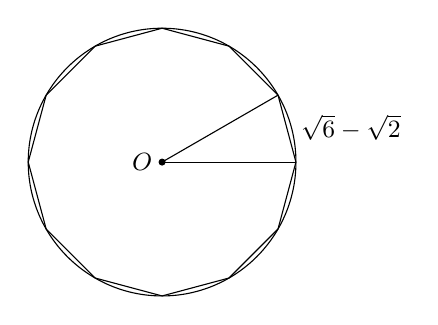
\begin{tikzpicture}[scale=0.85,font=\small]
\draw (0,0) circle (2); \draw (0:2) \foreach \a in {30,60,...,330} {--(\a:2)}--cycle;
\draw (0,0)--(0:2); \draw (0,0)--(30:2); \fill (0,0) circle (1.5pt); \node[left] at (0,0) {$O$};
\node[right] at (15:2) {$\sqrt6-\sqrt2$};
\end{tikzpicture}}
\AB{Aylana radiusini toping.}{Ön ikkiburçak yuzini toping.}}
\QQ{44}{Piramidaning asosi rombdan iborat. Rombning ötkir burçagi $30^\circ$ ga, unga içki çizilgan doira radiusi $\sqrt3$ ga teng. Piramidaning yon yoqlari asos tekisligi bilan $60^\circ$ li burçak hosil qiladi.
\qfig{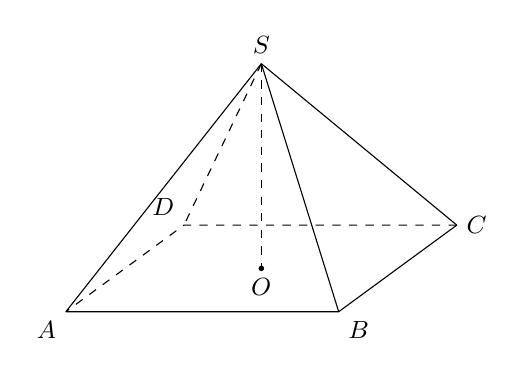
\begin{tikzpicture}[scale=0.5,font=\small]
\coordinate (A) at (0,0); \coordinate (B) at (6.93,0); \coordinate (C) at (9.93,2.2); \coordinate (D) at (3,2.2); \coordinate (O) at (4.965,1.1); \coordinate (S) at (4.965,6.3);
\draw (A)--(B)--(C); \draw[dashed] (C)--(D)--(A); \draw (S)--(A); \draw (S)--(B); \draw (S)--(C); \draw[dashed] (S)--(D); \draw[dashed] (S)--(O); \fill (O) circle (2pt);
\node[below left] at (A) {$A$}; \node[below right] at (B) {$B$}; \node[right] at (C) {$C$}; \node[above left] at (D) {$D$}; \node[above] at (S) {$S$}; \node[below] at (O) {$O$};
\end{tikzpicture}}
\AB{Piramidaning töla sirtini toping.}{Piramidaning hajmini toping.}}
\QQ{45}{Beşta işçi bir işni bajarmoqda. Birinçi, ikkinçi va uçinçi işçilar birgalikda işni $7{,}5$ soatda, birinçi, uçinçi va beşinçi işçilar $5$ soatda, birinçi, uçinçi va törtinçi işçilar $6$ soatda, ikkinçi, törtinçi va beşinçi işçilar $4$ soatda tugatadi.
\AB{Ikkinçi işçi yolğiz özi işni neça soatda tugatadi?}{Beşta işçi birgalikda işni neça soatda tugatadi?}}
\Javoblar{A B A A B D A D C D A B A B D C C D B A C D B B A B B B A C A B C E A}{\OK{36}{$3$}{$-3$}\OK{37}{$\dfrac\pi8$}{$8$}\OK{38}{$2\sqrt2\pi$}{$-\dfrac98$}\OK{39}{$3$}{$9$}\OK{40}{$\dfrac92$}{$\dfrac{49}3$}\OK{41}{$\dfrac{\sqrt2}2$}{$2+\sqrt3$}\OK{42}{$\dfrac7{\sqrt{65}}$}{$\dfrac{39}5$}\OK{43}{$2$}{$12$}\OK{44}{$72$}{$24$}\OK{45}{$20$}{$3$}}
